\documentclass{beamer}\usepackage[]{graphicx}\usepackage[]{color}
%% maxwidth is the original width if it is less than linewidth
%% otherwise use linewidth (to make sure the graphics do not exceed the margin)
\makeatletter
\def\maxwidth{ %
  \ifdim\Gin@nat@width>\linewidth
    \linewidth
  \else
    \Gin@nat@width
  \fi
}
\makeatother

\definecolor{fgcolor}{rgb}{0.345, 0.345, 0.345}
\newcommand{\hlnum}[1]{\textcolor[rgb]{0.686,0.059,0.569}{#1}}%
\newcommand{\hlstr}[1]{\textcolor[rgb]{0.192,0.494,0.8}{#1}}%
\newcommand{\hlcom}[1]{\textcolor[rgb]{0.678,0.584,0.686}{\textit{#1}}}%
\newcommand{\hlopt}[1]{\textcolor[rgb]{0,0,0}{#1}}%
\newcommand{\hlstd}[1]{\textcolor[rgb]{0.345,0.345,0.345}{#1}}%
\newcommand{\hlkwa}[1]{\textcolor[rgb]{0.161,0.373,0.58}{\textbf{#1}}}%
\newcommand{\hlkwb}[1]{\textcolor[rgb]{0.69,0.353,0.396}{#1}}%
\newcommand{\hlkwc}[1]{\textcolor[rgb]{0.333,0.667,0.333}{#1}}%
\newcommand{\hlkwd}[1]{\textcolor[rgb]{0.737,0.353,0.396}{\textbf{#1}}}%
\let\hlipl\hlkwb

\usepackage{framed}
\makeatletter
\newenvironment{kframe}{%
 \def\at@end@of@kframe{}%
 \ifinner\ifhmode%
  \def\at@end@of@kframe{\end{minipage}}%
  \begin{minipage}{\columnwidth}%
 \fi\fi%
 \def\FrameCommand##1{\hskip\@totalleftmargin \hskip-\fboxsep
 \colorbox{shadecolor}{##1}\hskip-\fboxsep
     % There is no \\@totalrightmargin, so:
     \hskip-\linewidth \hskip-\@totalleftmargin \hskip\columnwidth}%
 \MakeFramed {\advance\hsize-\width
   \@totalleftmargin\z@ \linewidth\hsize
   \@setminipage}}%
 {\par\unskip\endMakeFramed%
 \at@end@of@kframe}
\makeatother

\definecolor{shadecolor}{rgb}{.97, .97, .97}
\definecolor{messagecolor}{rgb}{0, 0, 0}
\definecolor{warningcolor}{rgb}{1, 0, 1}
\definecolor{errorcolor}{rgb}{1, 0, 0}
\newenvironment{knitrout}{}{} % an empty environment to be redefined in TeX

\usepackage{alltt}
\usepackage{blindtext}
\usepackage{longtable}
\usepackage{array,booktabs}
\usepackage{tikz}
\usepackage{animate}
\usepackage{outlines}
\usetheme{Execushares}

\title{A \LaTeX Workflow for MSDS}
\subtitle{An easy way to quickly get something nice to turn in}
\author{David Josephs}
\date{\today}

\setcounter{showSlideNumbers}{1}
\IfFileExists{upquote.sty}{\usepackage{upquote}}{}
\begin{document}

	\setcounter{showProgressBar}{0}
	\setcounter{showSlideNumbers}{0}

	\frame{\titlepage}

	\begin{frame}
		\frametitle{Contents}
		\begin{enumerate}[<+->]
			\item Introduction to \LaTeX \\ \textcolor{ExecusharesGrey}{\footnotesize\hspace{1em} Reasons to give up Word forever, bibtex, and demonstrations}
			\item A Single-Source \LaTeX Workflow  \\ \textcolor{ExecusharesGrey}{\footnotesize\hspace{1em} Integrating code and analysis into \LaTeX}
		\end{enumerate}
	\end{frame}

	\setcounter{framenumber}{0}
	\setcounter{showProgressBar}{1}
	\setcounter{showSlideNumbers}{1}
	\section{\LaTeX Primer}
		\begin{frame}
			\frametitle{What is \LaTeX?}
			\begin{outline}
\1 Document Preparation System
\2 Typesetting
			\end{outline}
		\end{frame}

		\begin{frame}
			\frametitle{Why \LaTeX?}
\begin{itemize}[<+->]
		\item Word is the worst
		\begin{itemize}
		\item Reproducibility
		\item Figures and tables
		\end{itemize}
		\item Separate style and body
		\item Control issues
		\begin{itemize}
		\item Ligatures
		\item Manipulate everything
		\end{itemize}
\end{itemize}
		\end{frame}
\begin{frame}
\frametitle{Using \LaTeX}
Recommendations for installation:
\begin{itemize}[<+->]
	\item \TeX distributions
	\begin{itemize} \item Mac: MacTEX
	\item Windows: MiKTeX or proTeXt
	\item Linux: \TeX  or TeXLive \end{itemize}
	\item \LaTeX editors
	\begin{itemize}
	\item LyX and Overleaf
	\item Mac: Texpad
	\item Windows: TeXStudio 
	\item Linux: TeXStudio
	\end{itemize}
	\end{itemize}
\end{frame}
\begin{frame}
\frametitle{Demonstration}
\begin{itemize}[<+->]
	\item{Creating a .tex file}
	\begin{itemize}
		\item Preamble (document class + package loading)
		\item Body
	\end{itemize}
\item \emph{Italics}, \textbf{Bold}, and \textsc{Small Cap}
\item{Sectioning and TOC}
\item{Math and mathpix}
\item Tables
\item Figures
\item Cross-References
\item Bibliography
\item Templates!
\end{itemize}
\end{frame}
	\section{Reproducible Research Using \LaTeX}
		\begin{frame}
			\frametitle{A Workflow Using knitr and \LaTeX}
			\begin{itemize}[<+->]
				\item .Rnw file extension
				\item Normal LaTeX preamble
				\item Set knitr chunk and engine options
				\item .Rnw $\rightarrow$ .tex $\rightarrow$ .pdf
			\end{itemize}
		\end{frame}
\begin{frame}
\frametitle{Chunky}
Chunk name and options are defined by '<< chunk name and options>> ' , followed by '=', then your code is included, then the chunk is punctuated with an '@'.
\end{frame}
		\begin{frame}
\frametitle{Making tables with knitr}
To make a table, you say chunk results='asis', and print an xtable
\end{frame}
		\begin{frame}
\frametitle{Making tables with knitr | Example}
\begin{kframe}
\begin{alltt}
\hlstd{WheatEater}\hlkwb{<-} \hlkwd{read.csv}\hlstd{(}\hlstr{"Data/Wheateater.csv"}\hlstd{)}

\hlstd{model1} \hlkwb{<-}\hlkwd{lm}\hlstd{(Tcell}\hlopt{~}\hlstd{Mass,}\hlkwc{data}\hlstd{=WheatEater)}

\hlstd{table1}\hlkwb{<-}\hlkwd{xtable}\hlstd{(model1,}
\hlkwc{label}\hlstd{=}\hlstr{'tb:model1'}\hlstd{,}

\hlkwc{caption}\hlstd{=}\hlstr{"Results of the Model"}\hlstd{)}

\hlkwd{print}\hlstd{(table1,}\hlkwc{booktabs}\hlstd{=T,}\hlkwc{table.placement}\hlstd{=}\hlstr{'H'}\hlstd{)}
\end{alltt}
\end{kframe}% latex table generated in R 3.5.1 by xtable 1.8-3 package
% Tue Nov 13 03:56:36 2018
\begin{table}[H]
\centering
\begin{tabular}{rrrrr}
  \toprule
 & Estimate & Std. Error & t value & Pr($>$$|$t$|$) \\ 
  \midrule
(Intercept) & 0.0875 & 0.0787 & 1.11 & 0.2800 \\ 
  Mass & 0.0328 & 0.0106 & 3.08 & 0.0061 \\ 
   \bottomrule
\end{tabular}
\caption{Results of the Model} 
\label{tb:model1}
\end{table}

\end{frame}
		\begin{frame}
\frametitle{Making figures with knitr}
To make a beautiful figure, you set your device to tikz (dev='tikz'), which produces an amazing, non-rasterized figure. Note on the first run through, this can take a while, which is why we cache our output.
\end{frame}
		\begin{frame}
\frametitle{Making figures with knitr | Example}
\begin{knitrout}
\definecolor{shadecolor}{rgb}{0.969, 0.969, 0.969}\color{fgcolor}\begin{kframe}
\begin{alltt}
\hlstd{resp}\hlkwb{<-}\hlkwd{ggplot}\hlstd{(model1,} \hlkwd{aes}\hlstd{(.fitted,.resid))}
\end{alltt}
\end{kframe}
\end{knitrout}
And so on. The next slide contains just basic ggplot output, but compiled using tikz into the pdf (with a surprise). 
\end{frame}
\begin{frame}
\frametitle{Making figures with knitr | Example}
\begin{figure}[H]
	\caption{An animated plot from ggplot2, in PDF form}
\begin{knitrout}
\definecolor{shadecolor}{rgb}{0.969, 0.969, 0.969}\color{fgcolor}




\animategraphics[,controls,loop]{1}{figure/plot1-}{1}{5}

\end{knitrout}
\end{figure}
\end{frame}
		\begin{frame}
			\frametitle{Integrating SAS}
			Integrating SAS is super easy. 
			\begin{itemize}[<+->]
				\item engine = 'sashtml'
				\begin{itemize}
					\item enginepath = sasexe
					\item engineopts = sasopts
				\end{itemize}
			\item SAS figures are exported as PNGs
			\begin{itemize}
				\item Call those in \LaTeX
			\end{itemize}
		\item SAS tables are exported as HTML
		\begin{itemize}
			\item Call with R library XML
			\item Print with xtable
		\end{itemize}
	\item SAS code does not save between chunks
	\begin{itemize}
		\item Clever echos
	\end{itemize}
		\end{itemize}
		\end{frame}
\begin{frame}
\frametitle{SAS Example}
\begin{knitrout}
\definecolor{shadecolor}{rgb}{0.969, 0.969, 0.969}\color{fgcolor}\begin{kframe}
\begin{alltt}
proc glm data=powermetabolism plots=all alpha=.05;
model Metab=powerMass / CLPARM;
run;
\end{alltt}
\end{kframe}
\end{knitrout}
\end{frame}
\begin{frame}
\frametitle{SAS Example}
 Alternatives For SAS University Edition
\begin{figure}[H]
	\label{fig:SASdiagraw}
	\begin{center}
		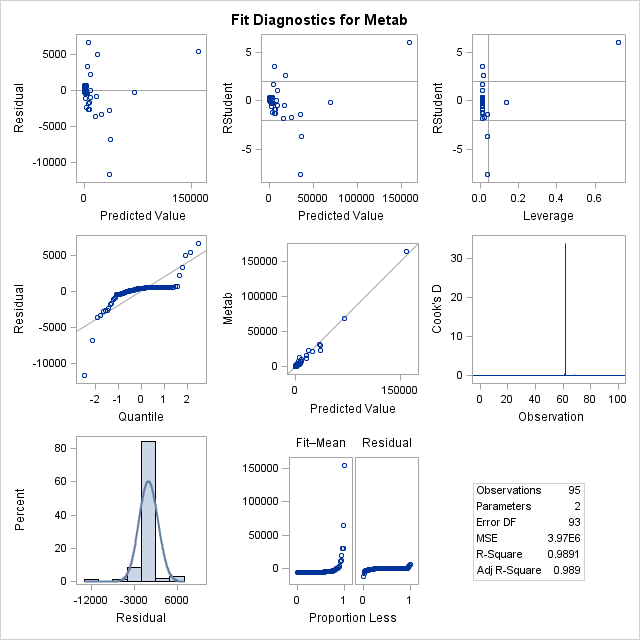
\includegraphics[scale=.25]{SASout/sasassraw.png}
	\end{center}
\caption{Diagnostic Plots on the Raw Metabolism Data}
\end{figure}
\end{frame}
\begin{frame}
\frametitle{Other Languages}
Knitr and LaTeX have full support of Python, C++, C, Java, and you can really easily add your own. I know python can be saved across chunks, and works with tikz
\end{frame}
	\section{Conclusions}
		\begin{frame}
			\frametitle{Closing Thoughts}
			\begin{itemize}[<+->]
				\item Don't use Word
				\item \LaTeX is fun
			\end{itemize}
		\end{frame}
\begin{frame}
\frametitle{Questions}
Thank you! 
\end{frame}
	\appendix
	\backupbegin
	  \begin{frame}
	    \frametitle{Backup slide 1}
	    \blindtext
	  \end{frame}
	\backupend

\end{document}
